\chapter{Theoretical Background}\label{chap:theorie}

This chapter will give an overview of wireless coexistence testing and fundamental test methods. This chapter explores a brief introduction to radiation test sites and the demand of the novel test approach. Subsequently,
this chapter presents the theory and equations of antenna properties and \acf{MU}.

\section{ Wireless Coexistence Testing  } 
Wireless devices mainly operate either in 2.4 GHz or 5 GHz \acf{ISM} band. Since the number of these interconnected devices is increasing, it becomes necessary to control the use of these bands. All wide-band transmission systems using these bands need to ensure their compliance with certain standards.  It ensures that one device is not impacting other wireless devices operating in the same band. \\

The method of measuring the ability of multiple devices to interact in a single environment with limited bandwidth is known as wireless coexistence testing. Coexistence, which is a natural outgrowth of \acf{EMC}, refers to ensuring one user's wireless device will not impact another wireless device and cope with the presence of signals from other devices (i.e. blocking signal). To comply with local and regional requirements, \acs{RF} regulatory testing is done to demonstrate that the products will use the radio spectrum effectively. Coexistence among wireless devices depends upon separation distance, frequency, space and time. The probability of coexistence increases as the frequency separation of channels increases between wireless networks, \acf{SIR} increases, overall channel occupancy of the two wireless networks decreases. \\

All countries in the world today have the authority to create and enforce technology regulations specific unto itself but most of the countries adopt such regulations that are uniform with other larger or technologically advanced countries. Countries sharing common borders share a common set of regulations and referred to in the 802.11 specification as regulatory domains. All of these domains have different parameters for antenna gain, transmit power, channel selection, etc. that must be followed. Additionally, many countries may follow a single standard in its entirety, or may use one of the standards set as a guideline and apply their own unique changes. Fortunately, only a few countries fall in the latter category today. Out of the vast technology regulations governing over the world, the only 4 major regulatory bodies that exercise authority over the world's technology regulations are mentioned in the following sub-sections (referred from \cite{ppr_2020}).

\subsection{\acf{FCC}}
The first regulatory bodies to police spread spectrum and \acsp{WLAN} were the \acf{FCC} and  \acf{IC}, which have jurisdiction over the United States and Canadian \acs{RF} regulations, respectively. Although referred to as the \acs{FCC} domain in the 802.11 specifications, the \acs{FCC} and \acs{IC} are commonly called the North American regulatory domain. \\

Geographical areas where the \acs{FCC} regulatory domain is used are: North America (including Canada), Central America, South America, Australia, New Zealand, Hong Kong, India, Malaysia, Philippines, Taiwan and Parts of the Russian Federation.

\subsection{\acf{ETSI}}
\acs{ETSI} is more of an advisory body than a regulatory body (unlike the \acs{FCC} and\acs{TELEC}), and makes recommendations for regulations instead of enacting them itself. As the name implies, the \acs{ETSI} was developed with the European countries in mind; however, many other countries worldwide follow the \acs{ETSI} recommendations. Geographical areas where the \acs{FCC} regulatory domain is used are: Europe, Middle East, Africa, China, Indonesia, Singapore, Thailand, Vietnam and Parts of the Russian Federation. \\

\acs{ETSI} EN 300 328 is a European harmonized standard that specifies the regulatory requirement for data transmission equipment operating in the 2.4 GHz \acs{ISM} band and using wide-band modulation techniques in Europe. The standard specifies \acfp{KPI} that can be used to assess the ability of the \acs{DUT} to coexist with other device in the intended operational environment (\cite{7927764}). This standard covers technologies such as Wi-Fi\texttrademark{}, Bluetooth\textregistered{} and ZigBee but also other proprietary transmission systems that use the 2.4 GHz \acs{ISM} band.  \\

In this thesis, I would use V2.1.1 of the mentioned standard. There are about 7 to 8 tests per standards. However, the test cases that I planned to use for the normalized measurements are:
\begin{itemize}
\item \acf{OBW} \cite{etsi300328}: It is defined as the bandwidth that contains 99 \% of the power of the signal. The limits depend on the specification of the \acs{DUT}. The limits are taken from the respective standards.
\item Receiver Blocking \cite{etsi300328}:  Measure of the capability of the equipment to receive a wanted signal on its operating channel without exceeding a given degradation due to the presence of an unwanted input signal (blocking signal) on frequencies other than those of the operating bands provided in the standard. The minimum performance criterion is defined to be a \acf{PER} of less than or equal to 10 \%.
\item \acf{PSD} \cite{etsi300328}: It is the mean equivalent isotropically radiated power (\acs{EIRP}) spectral density in a 1 MHz bandwidth during a transmission burst. The limits depend on the specification of the \acs{DUT}. The limits are taken from the respective standards.
\end{itemize}
Spurious measurements are not supported because normalization is done for the in-band frequencies and thus gain of antenna is not known. In-order to perform these measurements, out-of-band calibration needs to be done for the test system. 


\subsection{\acf{TELEC}}
In Japan, the \acf{TELEC}, part of the Japanese Ministry of Posts and Telecommunications, defines the regulations for \acs{WLAN} and other radio services. The \acs{TELEC} regulatory domain is used only in Japan.


\subsection{\acf{KCC}}
\acs{KCC} is a South Korean media regulation agency modelled after the \acf{FCC} of the United States of America. It was established on February 29, 2008. The \acs{KCC} regulatory domain is used only in Korea.
 

\section{Fundamental Coexistence Test Methods}
Coexistence testing approaches are mainly categorized into three approaches: conducted testing, radiated controlled environment (e.g. \acsp{AC}), or radiated open environment. The test method selected can be a combination of all the 3 categories above, but the location of the \acs{DUT} will determine one of these three approaches as the distinguishing feature. Some of the advantages and disadvantages of the coexistence testing approaches are described as below (referred from \cite{gonzalez}).

\subsection{Conducted Testing}
Conducted test methods comprises of a configuration of \acs{RF} cables, combiners, couplers, etc. to establish communication channels between the various wireless transceivers. Conducted measurements are cost effective, easy to setup and have a lower \acf{MU}.

\subsection{Radiated Controlled Environments}
A radiated controlled environment consists of non-reflective chambers (e.g. \acsp{AC}) which provides a calibrated field at the location of the \acs{DUT}. The main advantage of this approach is that antennas used during actual operation are included in the test, radiated path loss is well controlled and shielding effectively eliminates chances of potential interference. Most \acsp{DUT} these days come with an integrated antenna and hence options of cable connectors may not be available anymore. Even if such a connection port does exist, then the use of a radiated controlled environment might be beneficial as the setup will include the antenna impacts, such as pattern, mismatch, and efficiency in the test which is not included in conducted method.

\subsection{Radiated Open Environment}
The radiated open environment approach performs a coexistence test by using a deployed system in an actual room. In this approach, ambient \acs{RF} conditions are monitored during testing to ensure the test is not corrupted by extraneous signals. This configuration enables testing without the need for a chamber. It also represents a \acf{NLOS} configuration that is not directly achievable in either of the two previously discussed methods. Thus, it is possible to realize a time delay spread in communication channel. While the average path loss impacts of the \acs{NLOS} can be accounted for by the attenuation in the two previous methods, this third method can be viewed as a more realistic setup for \acs{RF} propagation considerations. Similar to the radiated controlled environment, the \acs{DUT} antennas are included in the test. 

 

\section{Measurement Grids}
In the cylindrical scanning technique, illustrated in Figure \ref{fig:cs}(a). The azimuthal location of the antenna is held constant while the fields are probed at discrete locations in the vertical direction at some fixed distance from the antenna. At the completion of each vertical scan, the test antenna is rotated to the next angular position. A spherical scan can be accomplished by fixing the location and orientation of the probe and varying the angular orientation of the test antenna with a dual-axis positioner, as shown in Figure \ref{fig:cs}(b) \cite{balanis}. 

\begin{figure}[H]
\centering
  \subfigure[Cylindrical]{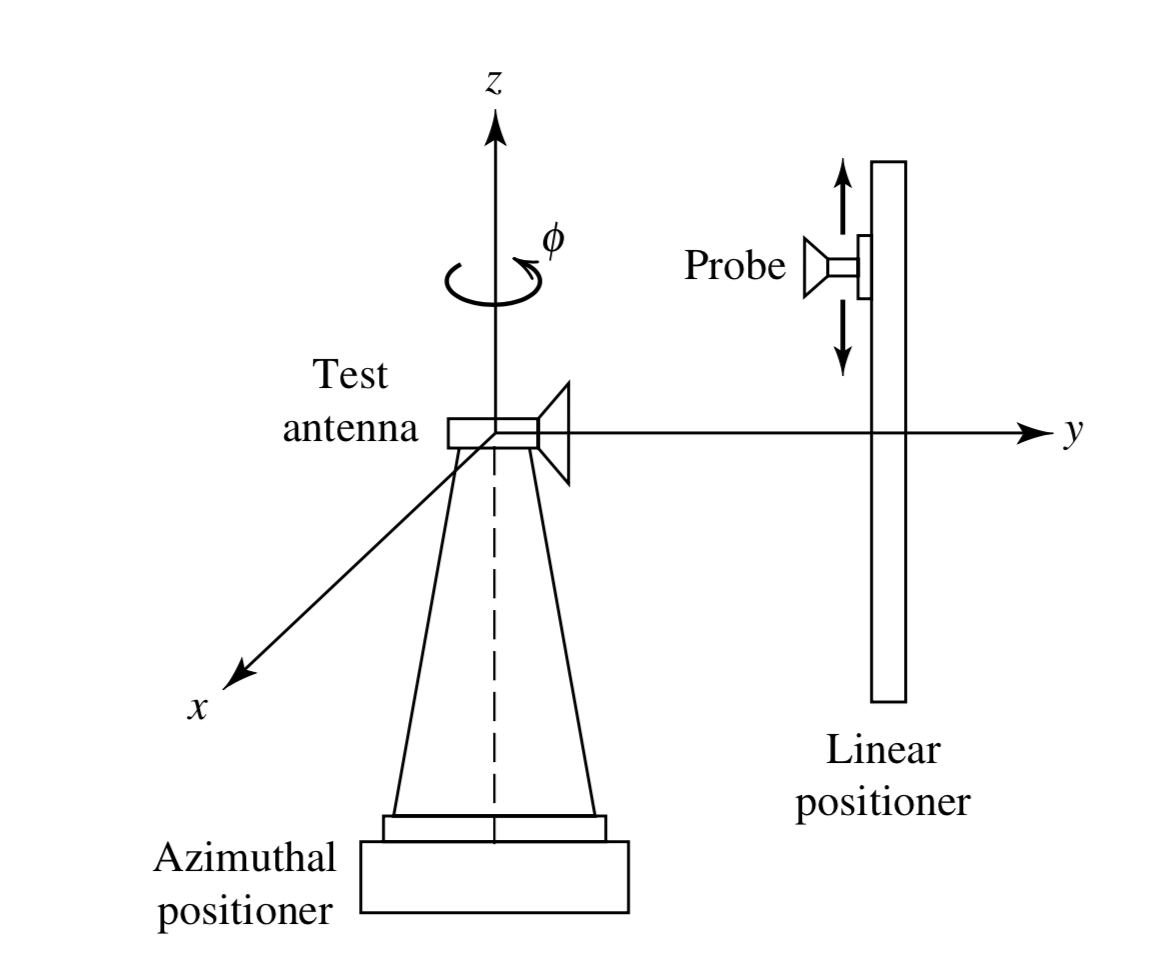
\includegraphics[width=0.45\textwidth]{cyl_grid.png}} 
  \subfigure[Spherical]{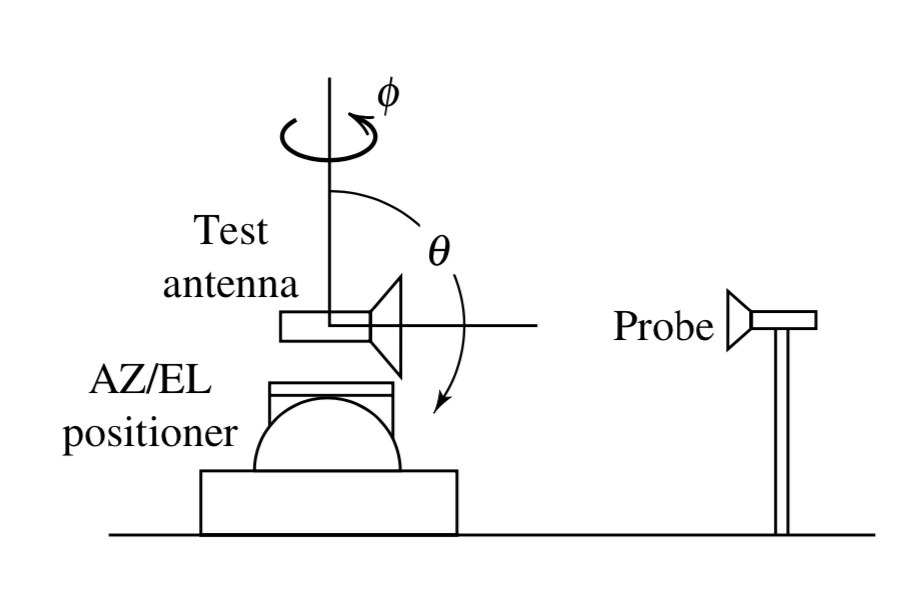
\includegraphics[width=0.45\textwidth]{spherical_grid.png}}
\caption{Schematic representation of typical cylindrical and spherical surface positioning systems \cite{balanis}}
\label{fig:cs}
\end{figure}

According to the standard, for the reference (\acs{EIRP}) measurement, a cylindrical grid should be used. A cylindrical scan is easier to implement and common in existing Electromagnetic Interference (EMI) chambers. Nevertheless, there is a risk that the maximum \acs{EIRP} can be missed easily depending on the placement of the \acs{DUT}. Therefore a spherical grid is more logical instead of using a cylindrical grid mentioned in the standard \cite{etsi300328}. This measurement can be done using \acs{RS} ATS1000 antenna test chamber or \acs{RS} Wireless Performance Test Chambers (WPTC).


\section{Wireless Coexistence Testing using \acs{RS}\textregistered{} Regulatory Test System}
The approach is based on \acs{RS}\textregistered{} TS8997 Regulatory Test System for wireless coexistence testing. This system already includes a vector signal generator, a spectrum analyzer and switching modules which is required to perform conducted measurements for regulatory tests mentioned in \acs{ETSI}, \acs{FCC} standards. This thesis investigates the approach of normalized measurements using the \acs{RF} shielded box along with a switching module used to switch between the probe antennas placed within the \acs{RF} shielded box, which actually is the extension of the current regulatory test system. As a result of increase in test cases, it is an advantage to have a procedure of specialized test system and special wireless automated test. Normalization calibrates the resulting values measured within the \acs{RF} Shielded Box with the measured maximum \acs{EIRP} value from the \acs{AC}. Chapter \ref{chap:normalized} explains this novel technique in detail.

\section{Antenna Fundamentals}
For this work, a close understanding of the theory of the used antennas and their radiations is needed in-order to explain and analyze the physics happening inside of the test system and influencing the measurements in the chamber. To describe the performance of antennas, the definition of various parameters is necessary. The following sub-sections highlights some important antenna parameters.

\subsection{Radiation Patterns}
One trace of the electric or magnetic field of a considered type of antenna at a constant radius is called the amplitude field pattern. In addition, the spatial variation of the power density along a constant radius can be studied on a graph called the amplitude power pattern. The field and power patterns are usually normalized with respect to their maximum value, yielding normalized field, and power patterns. To accentuate more the details of the pattern with very low values, usually referred to as minor lobe (Figure \ref{spherical}) the power pattern plot is computed on a logarithmic scale or more commonly in decibels (dB). \\

A radiation pattern represents the three-dimensional variation of the power radiated by an antenna as a function of the direction away from the antenna. In most cases, the radiation pattern is determined in the \acs{FF} region and is represented as a function of the directional coordinates (Figure \ref{spherical}). Radiation properties include power flux density, radiation intensity, field strength, directivity, phase, or polarization \cite{balanis}. Different antennas can be classified depending on the characteristics of their patterns. A pattern is called isotropic if the radiation is the same in all directions, which is not realizable in practice but useful for comparison to real antennas. Some antennas may also be described as omnidirectional, which means that the radiation pattern is isotropic in one single plane, for example, the dipole antenna and the slot antenna. The third category of antennas is the directional antennas, also called beam antennas. The peak represents the direction where the bulk of the radiated power travels. Directional antennas are very common, examples of antennas with highly directional radiation patterns include the dish antenna and the slotted waveguide antenna. The measurements achieved in this work use six \acs{RS}\textregistered{} vivaldi antennas as probe antennas, and omni-directional antennas for the \acs{DUT}. \\

While the radiation pattern is actually three-dimensional, it is common however to describe this behaviour with two planar patterns, also called the principal plane patterns. The horizontal pattern, which describes the field strength as a function of the azimuth angle $\phi$  with a fixed elevation angle $ \vartheta$. And the vertical pattern, which describes the field strength as a function of the elevation angle $\vartheta$  for a fixed azimuth angle $\phi$. These patterns are commonly referred to as azimuth pattern and elevation pattern. The term azimuth describes the reference to the horizontal while the term elevation describes the reference to the vertical. The spherical coordinates as shown in figure \ref{spherical} are commonly used to describe a location in the three-dimensional space.

%%%%%%%%%%%%%%%%%%%% Figure Spherical %%%%%%%%%%%%%%%%%%%%
\begin{figure}[H]
	\begin{center}
	\vspace{-1cm}
		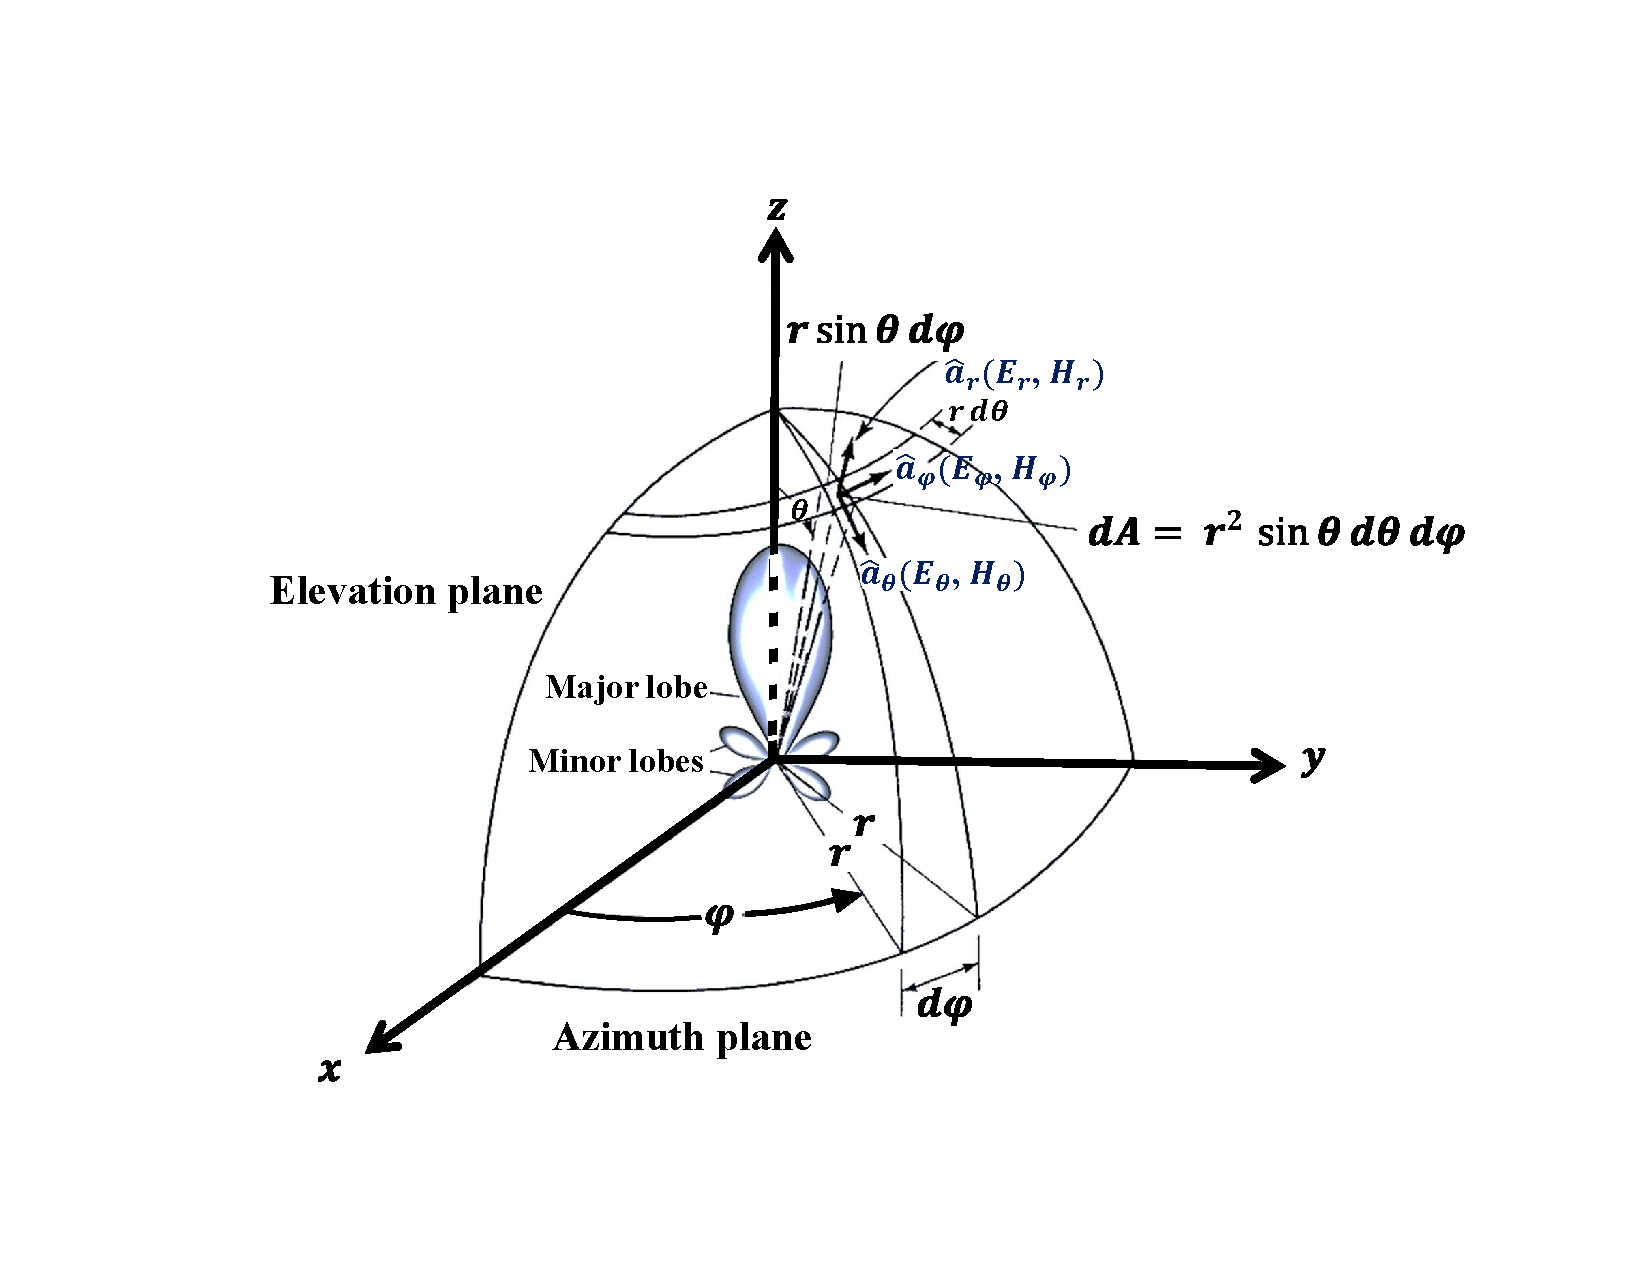
\includegraphics[width=0.95\textwidth]{spherical.pdf}
			\vspace{-1cm} 	\caption{\label{spherical}Spherical co-ordinates for antenna analysis \cite{balanis}}
	\end{center}
\end{figure}

\subsection{Directivity}

Isotropic antennas are theoretical point sources that spread electromagnetic energy equally in all directions. The total radiated power is determined by integrating the power flux density over the surface of a sphere of radius $r$ that surrounds the antenna. The integral represents the theoretical total radiated power. As the distance from the source increases, the surface area of the integrating sphere increases in proportion to the square of the radius of the sphere. The energy from isotropic emitters spreads out evenly to cover this increasingly larger area, and thus the electromagnetic power flux density decreases in proportion to the square of the distance from the source.
The directivity  $D$  of an antenna is the maximal value of its directive gain. Directive gain is represented as  $D \left(  \theta , \varphi  \right)$  and compares the radiant intensity  $U \left(  \theta , \varphi  \right)$  defined as the power per unit solid angle that an antenna creates in a particular direction against the average value over all directions:
\begin{equation}
D \left(  \theta , \varphi  \right) = \frac{ U \left(  \theta , \varphi  \right) }{P_{tot}/ \left( 4 \pi  \right) } \quad  \mbox{where} \quad  P_{tot}= \int_{ \varphi =}^{ \varphi =2 \pi } \int_{ \theta =0}^{ \theta = \pi }U\sin  \theta d \theta d \varphi.
\label{directivity}
\end{equation}

Directivity is defined as the maximal directive gain value found among all possible solid angles, it is then the ratio of the power density of the physical antenna in its most concentrated direction to that of a theoretical isotropic emitter of the same total power transmission level with a maximum value of 1 (0dB).

\begin{equation}
D_{0} = \mbox{max} \left( \frac{~U \left(  \theta , \varphi  \right) }{\frac{P_{tot}}{4 \pi }} \right) ~=\frac{~  U \left(  \theta , \varphi  \right)  \vert_{\max }}{\frac{1}{4 \pi } \int_{0}^{2 \pi } \int _{0}^{ \pi }U \left(  \theta , \varphi  \right) \sin  \theta d \theta d \varphi }.
\end{equation}




%%%%%%%%%%%%%%%%%%%% Figure 2Dpattern %%%%%%%%%%%%%%%%%%%%

%\begin{figure}[H]
%	\begin{center}
%		\includegraphics[width=1\textwidth]{./media/image2.png}
%					\caption{\label{2Dpattern} Two-dimesional directivity pattern of a $\lambda /2$ dipole \cite{balanis}}
%	\end{center}
%\end{figure}



\subsection{Efficiency}

The total antenna efficiency considers losses at the input terminals and within the structure of the antenna. The total efficiency of an antenna is the radiation efficiency multiplied by the impedance mismatch loss of the antenna, when connected to a transmission line or receiver so that the total efficiency can be computed as:
\begin{equation}
e_{total}= e_{ref} \cdot e_{cd}= e_{cd} \left( 1- \vert  \Gamma  \vert ^{2} \right).
\end{equation}

Where $e_{total}$ is the total efficiency, $e_{ref}$ is the reflection or mismatch efficiency, $e_{cd}$ is the radiation efficiency which is the product of the conduction efficiency and the dielectric efficiency. This antenna radiation efficiency quantifies the actual losses of a particular antenna design due to many factors such as manufacturing faults, impedance mismatch, surface coating losses, or other factors. It is computed as the ratio of the radiated power to the input power of the antenna and its value lies between 0 and 1 or as a percentage. $\Gamma$ is the voltage reflection coefficient at the input terminals of the antenna:  $\Gamma =\frac{ \left( Z_{in~}- Z_{0~} \right) }{ \left( Z_{in~}+ Z_{0~} \right) }$\  where  $Z_{in}$ is the input impedance of the antenna and  $Z_{0}$ is the characteristic impedance of the transmission line.

\subsection{Gain}
The antenna gain describes how much power is transmitted in the direction of peak radiation to that of an isotropic source. If the antenna is supposed to have for example, 3dB gain, this means that the received power should be 3dB higher than the power that is received at the same input power by an isotropic antenna. Antenna gain incorporates both directivity and efficiency of the antenna so that the gain is computed as the product of both values: 

\begin{equation}
G \left(  \theta , \varphi  \right) =e_{cd} \left[ \frac{~U \left(  \theta , \varphi  \right) }{\frac{P_{tot}}{4 \pi }} \right]
\end{equation}



\subsection{Field Regions}
The space around an antenna is usually sub-divided into three regions, reactive near-field region, radiating near-field also called Fresnel region and far-field also called Fraunhofer region. Figure \ref{regions} shows changes of antenna amplitude pattern shape in the different field regions \cite{7942128}. \\

The closest region to an antenna, with dimensions defined as following: $d \ll $ $ \lambda $  , is termed the near field and is dominated by magnetic fields. A transition zone exists for one to two wavelengths, and then there is the far-field region of an antenna, for which the dimensions are: $d>2\lambda $  , where the electric field becomes dominant.

In far field \acs{RF} link the ratio between the received and transmitted power can be defined as \cite{schantz}:
\begin{equation}
\frac{P_{RX}}{P_{TX}}=\frac{G_{TX}G_{RX}}{4 \left( kr \right) ^{2}}=\frac{G_{TX}A_{RX}}{4 \pi r^{2}}=\frac{A_{TX}A_{RX}}{ \lambda ^{2}r^{2}} \quad %\cite{schantz}.
\end{equation}
The effective area A, also called aperture of an antenna, is related to gain as follows: 
\begin{equation}
A=\frac{ \lambda ^{2}G}{4 \pi }
\end{equation}

In the near-field, the formula diverges into two different formulas, one for links that are the same (like), either both magnetic or both electric, and one different formula that describes different links (unlike). In the experiments in this work we only consider electric antennas (like). The ratio is than expressed as following \cite{schantz}:

\begin{equation} \label{eq:near}
\frac{P_{Rx}}{P_{Tx}}=\frac{G_{Tx}G_{Rx}}{4} \begin{array}{c}
	 \left( \frac{1}{ \left( kr \right) ^{6}}-\frac{1}{ \left( kr \right) ^{4}}+\frac{1}{ \left( kr \right) ^{2}} \right) ~like~\\
	 \left( \frac{1}{ \left( kr \right) ^{4}}+\frac{1}{ \left( kr \right) ^{2}} \right) ~unlike\\
	\end{array} \quad %\cite{schantz}.
\end{equation}

%%%%%%%%%%%%%%%%%%%% Figure/Image No: 4 starts here %%%%%%%%%%%%%%%%%%%%
%
\begin{figure}[H]
\centering
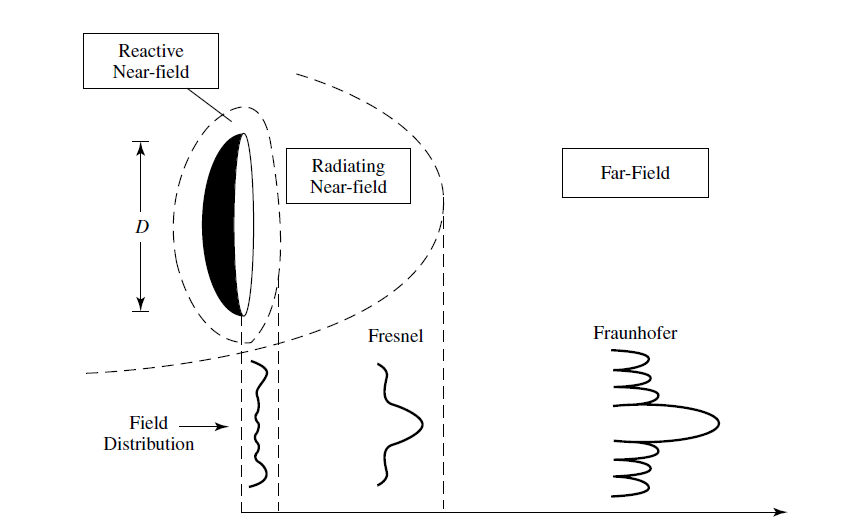
\includegraphics[scale = 0.5]{image4.png}
\caption{\label{regions} Field regions of an antenna \cite{balanis}}
\end{figure}


%%%%%%%%%%%%%%%%%%%% Figure/Image No: 4 Ends here %%%%%%%%%%%%%%%%%%%%


\subsection{\acf{FSPL}}
When there is an unobstructed direct line-of-sight path between the antennas for transmitting and receiving, it is possible to estimate the received signal and the link budget. The characterization of the average path loss experienced in a wireless channel helps to estimate the received signal. The average path loss is defined as the amount of loss experienced in a propagation environment as a function of the transmitter-receiver distance. The received power for free-space propagation can be expressed by the Friis free space equation expressed by the following formula \cite{schantz}:
\begin{equation}
P_{r} \left( d \right) = P_{t}\frac{G_{t}G_{r} \lambda ^{2}}{ \left( 4 \pi  \right) ^{2}d^{2}} 
\end{equation}
where, $d$ is the separation distance between the antennas,  $P_{t}$ is the transmitter power, $P_{r}$ is the received power as a function of the distance, $G_{t}$ the transmitter antenna gain, $G_{r}$ the receiver antenna gain and $\lambda$ the wavelength of the signal in meters. \\

The path loss ($PL$) which represents the signal attenuation is the ratio between the transmitted power and the received power and are usually measured in dB. The path loss in free-space in dB is given as the following sum, this formula means that higher separation and higher frequency result in higher attenuation:

\begin{equation} 
PL \left( d \right) =10\log(\frac{P_{t}}{P_{r}})  =20\log \left( \frac{4 \pi d}{ \lambda } \right) -G_{t}-G_{r}.
\end{equation}

\subsection{\acf{EIRP}}
\acs{EIRP} is the measured radiated power in a single direction for a fixed angle. It is expressed in the formula \ref{eirp}, where $P_{t}$ is the output power at the transmitter (in dBm), $\mbox{Loss}_{\mbox{c}}$ the cable signal loss caused by the cable from the transmitter circuit to the antenna and possibly including antenna mismatch (in dB) and $\mbox{Gain}_{\mbox{a}}$ is the antenna gain (in dBi).
\begin{equation}
\mbox{EIRP} =  P_{t} - \mbox{Loss}_{\mbox{c}}+  \mbox{Gain}_{\mbox{a}}. \label{eirp}
\end{equation}
  
  


\subsection{Polarization and Polarization Mismatch} \label{sec:pol}
The direction of oscillation of the electric field component of an electromagnetic wave describes the polarization of an antenna. When a radio wave is propagating in a medium, it is called the polarization of the radio wave. Linear polarization means that the electric field vector remains on the same plane all the time, it is considered a special case of elliptical polarization. There are horizontally or vertically polarized radiations, for example omni-directional are always vertically polarized. Circular polarization means that the electric field vector is rotating circularly about the direction of propagation for each \acs{RF} cycle. The polarization is a design choice during the \acs{RF} system design. \\

The difference between the polarization of the receiving antenna and the polarization of the incident wave results in the polarization mismatch, also characterized by the \acf{PLF} or the polarization efficiency which is the loss of the electromagnetic power due to this polarization mismatch. When receivers and transmitters antennas are not aligned there will be a reduction in power transfer between the two antennas and the amount of extracted power from the incoming signal will not be at its maximum. The \acs{PLF} has a maximum of 1 (0 dB) which means there is no polarization loss and that the receiver antenna receives all the intended incident power of the wave. While a \acs{PLF} of 0 ( $ -\infty $dB) means that there is a total polarization loss and the antenna at the receiver is unable to capture the incident power. Thus  $0<\acs{PLF}<1$. In order to calculate the \acs{PLF}, we first look at the far zone of the transmitting antenna, and consider its transmitted electromagnetic field by its components in the transmitter's local spherical coordinate system. The direction of the field is specified by the azimuth and elevation of the receiving antenna in the transmitter's local coordinate system (Figure \ref{pollos}). So that the polarization of the transmitter's antennas may be expressed as following:
\begin{equation}
E_{i}= E_{i,H}\hat{e}_{az}+ E_{i,V}\hat{e}_{el}= \widehat{ \rho _{w}}E_{i} \label{eq_pollos}
\end{equation} 
where $E_{i,H}$ and  $E_{i,V}$  are the horizontal and vertical components and  $\widehat{ \rho _{w}}$ is the unit vector of the incident wave. Equivalently, we express the polarization of the receiving antennas with respect to the spherical basis vectors at the receiver's local coordinate system:  
\begin{equation}
E_{r}= E_{r,H}\widehat{e^{'}}_{az}+ E_{r,V}\widehat{e^{'}}_{el}= \widehat{ \rho _{a}}E_{r}
\end{equation}
where,  $E_{r,H}$ and $E_{r,V}$ are the horizontal and vertical components and $\widehat{ \rho _{a}}$ is the unit vector of the receiving antenna. The \acs{PLF} may be computed as the dot product of the normalized transmitted and the received polarization vectors in the corresponding coordinates systems after being converted to the global coordinate system:
\begin{equation}
\rho =\frac{ \vert E_{i}E_{r} \vert ^{2}}{ \vert E_{i} \vert ^{2} \vert E_{r} \vert ^{2}}=  \vert \widehat{ \rho _{w}}\widehat{ \cdot  \rho _{a}} \vert ^{2}=  \vert \cos  \varphi _{P} \vert ^{2}
\end{equation}
where $\varphi _{P}$ is the angle between the two polarization unit vectors.
\begin{figure}[H]
\vspace{-1cm} 
	\begin{center}
		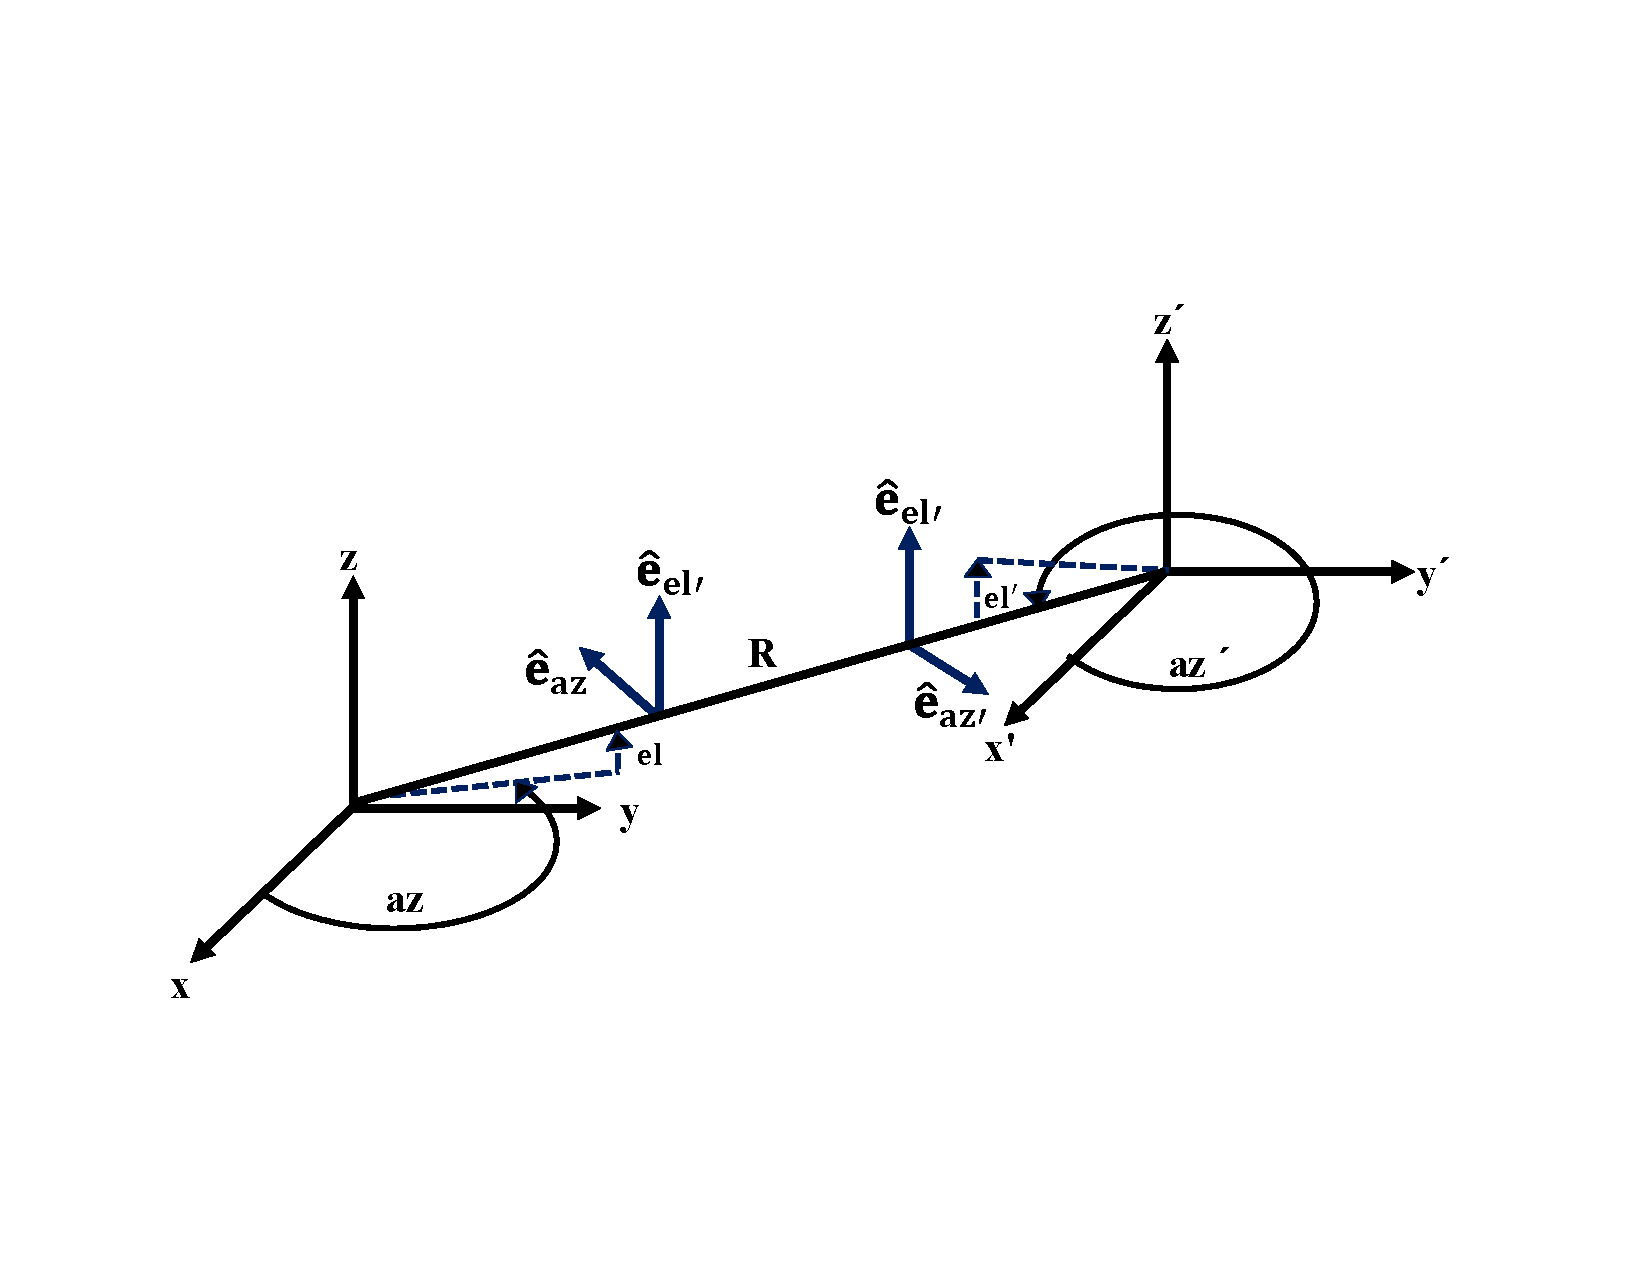
\includegraphics[width=1\textwidth]{pollos.pdf}
	\vspace{-2cm} 	\caption{\label{pollos} Local coordinates systems of tranmitter's and receiver's antennas for polarization loss calculation}
	\end{center}
\end{figure}


\subsection{Link Budget}
The link budget is a summary of the transmitted power considering all the gains and losses in the system and this enables the strength of the received signal to be estimated. The knowledge of the link budget is helpful for survey tools and measurements, because the expected values and the measured or observed value may differ from the originally transmitted or expected value. The link budget explains the values of the signal strength at the receiver input. A typical link budget formula for radio communications is:
\begin{equation}
P_{RX}= P_{TX~}+G_{TX}+ G_{RX}-L_{TX}-L_{RX}-L_{FSPL}-L_{P} \label{link_budget}
\end{equation}
where $P_{RX}$ is the received power in dBm, $P_{TX}$ is the transmitter output power in dBm, $G_{TX}$ and $G_{RX}$ the transmitter and receiver antenna gain in dBi, $L_{TX}$ and $L_{RX}$ the transmit and receiver feeder losses, $L_{FSPL}$ the free space path loss in dB and $L_{P}$ describes the propagation losses including polarization mismatch or medium losses.

\subsection{Bandwidth}
The bandwidth of an antenna is the range of frequencies over which the antenna can operate correctly. In other words, the performance of the antenna conforms to some standard with respect to certain specified characteristics, such as input impedance, beam width, gain, radiation efficiency and beam direction which all should be within an acceptable value of that of the center frequency. The bandwidth of the antenna can also be described in terms of percentage of the center frequency $F_{C}$ of the band or a ratio between the upper and lower frequencies $F_{H}$  and $F_{L}$ for broadband antennas as: 
\begin{equation}
BW=100  \times \frac{F_{H}-F_{L}}{F_{C}}
\end{equation}
%\textbf{2.2.12 Diversity and Beamforming and max ratio combining }


\section{\acf{MU}}
\acf{MU} is a quantitative indication of measurement results quality which allows values comparison among the same measurement or to reference values. This work investigates the novel approach of normalized measurements, and compares it, in terms of accuracy to its conducted alternatives. For the sake of making the results of measurements of physical quantities easy to asses we need some indications so that measurement results can be compared, either among themselves or with respect to values specified in standards and this is what we refer to as measurement uncertainties. \\

In this section the most used methodologies for the evaluation of measurement uncertainty are explained. There are two different types of \acs{MU} evaluation: Type A which is defined as $``$the method of evaluation of uncertainty by the statistical analysis of series of observations$"$ \cite{jcgm}.
The purpose of the Type A and Type B classification is to indicate the two different ways of evaluating uncertainty components and is for convenience of discussion only. Both types of evaluation are based on probability distributions and the uncertainty components are usually quantified by variances or standard deviations.
Evaluating type A uncertainty is achieved using:
\begin{itemize}
	\item Arithmetic mean:  $\overline{x}=\frac{1}{n} \sum _{i=1}^{n}x_{i}$.

	\item Standard deviation: $\sigma = \sqrt[]{\frac{1}{n-1} \sum _{i=1}^{n} \left( \overline{x}-x_{i} \right) ^{2}}$.

	\item Standard uncertainty.

	\item Degrees of Freedom: $``$The number of values in the final calculation of a statistic that are free to vary$"$  with the form  $\vartheta =n-1$.
\end{itemize}
Type B evaluation of uncertainty is defined as $``$the method of evaluation of uncertainty by means other than the statistical analysis of series of observations$"$ \cite{jcgm}. Essentially, type B uncertainty is data collected from anything other than an experiment performed by you. For example, datasheets, white papers, industry guides, calibration reports or other available information.